\documentclass[11pt,letterpaper]{article}
\usepackage[utf8]{inputenc}
\usepackage[T1]{fontenc}
\usepackage[spanish,es-nodecimaldot]{babel}
\usepackage{amsmath,amssymb}
\usepackage{geometry}
\usepackage{graphicx}
\usepackage{booktabs}
\usepackage{float}
\usepackage{listings}
\usepackage{xcolor}
\geometry{margin=2.3cm}
\setlength{\parskip}{4pt}

\lstset{basicstyle=\ttfamily\small, frame=single, columns=fullflexible,
        keywordstyle=\color{blue!70!black}, commentstyle=\color{green!40!black},
        breaklines=true}

\newcommand{\tsd}{0.30}
\newcommand{\zetad}{1}
\newcommand{\wnd}{13.3333}
\newcommand{\pthree}{66.6667}
\newcommand{\PdsA}{93.3333}
\newcommand{\PdsB}{1955.5556}
\newcommand{\PdsC}{11851.8519}
\newcommand{\Kp}{7.9136}
\newcommand{\Ki}{70.3792}
\newcommand{\Kd}{0.2759}
\newcommand{\KdT}{27.5911}
\newcommand{\KiT}{0.7038}
\newcommand{\qcdA}{36.2085}
\newcommand{\qcdB}{-63.0957}
\newcommand{\qcdC}{27.5911}
\newcommand{\PzA}{-1.750347}
\newcommand{\PzB}{0.765928}
\newcommand{\alfa}{0.513417}
\newcommand{\ezwT}{0.875173}
\newcommand{\dA}{-2.777181}
\newcommand{\dB}{2.826841}
\newcommand{\dC}{-1.247868}
\newcommand{\dD}{0.201897}
\newcommand{\ADA}{-2.576343}
\newcommand{\ADB}{2.202158}
\newcommand{\ADC}{-0.625815}
\newcommand{\qddA}{8.5234}
\newcommand{\qddB}{-14.3710}
\newcommand{\qddC}{6.1235}
\newcommand{\sdd}{-0.262282}
\newcommand{\oneMinusSdd}{1.262282}
\newcommand{\Umax}{57.9}
\newcommand{\Umin}{-44.7}
\newcommand{\maAts}{0.315}
\newcommand{\maAmp}{0.00}
\newcommand{\maAess}{0.000}
\newcommand{\maAise}{0.447}
\newcommand{\maBts}{0.315}
\newcommand{\maBmp}{0.00}
\newcommand{\maBess}{-0.000}
\newcommand{\maBise}{1.787}
\newcommand{\mbAts}{0.157}
\newcommand{\mbAmp}{1.68}
\newcommand{\mbAess}{-0.005}
\newcommand{\mbAise}{0.861}
\newcommand{\mbBts}{0.329}
\newcommand{\mbBmp}{2.89}
\newcommand{\mbBess}{-0.001}
\newcommand{\mbBise}{3.975}
\newcommand{\mcAts}{0.382}
\newcommand{\mcAmp}{0.12}
\newcommand{\mcAess}{0.000}
\newcommand{\mcAise}{1.270}
\newcommand{\mcBts}{0.360}
\newcommand{\mcBmp}{0.04}
\newcommand{\mcBess}{0.000}
\newcommand{\mcBise}{5.373}


\title{Discretización de la planta y diseño de controladores discretos\\
       \large Laboratorio 5 -- Control en discreto de un sistema mecánico}
\author{Control Lineal y Laboratorio -- Ingeniería en Mecatrónica, UMNG}
\date{}

\begin{document}
\maketitle

%--------------------------------------------------------------------------
\section{Planta continua identificada}

La planta es una masa (cremallera) movida por un motor DC con piñón de radio
$r = 9.4$~mm y sujeta por dos resortes $k_1$, $k_2$ con fricción viscosa $B$.
Del modelo físico,
\begin{equation}
  \frac{X(s)}{V(s)} = \frac{K_t/(R\,r)}{M_{eq}\,s^2 + B_{eq}\,s + (k_1+k_2)},
\end{equation}
es decir, un sistema de segundo orden sin ceros. A partir de diez pruebas de
escalón ($\pm60,\pm70,\pm80,\pm90,\pm100$~\% de PWM, muestreo de 10~ms, encoder
de $0.0671$~mm/cuenta) y estimación con \texttt{tfest} se obtuvo
\begin{equation}
  \boxed{G(s) = \frac{X(s)}{U_{ef}(s)} = \frac{168.4}{s^2 + 46.87\,s + 622.9}
  \quad \left[\frac{\text{mm}}{\%}\right]}
  \label{eq:Gs}
\end{equation}
donde la entrada es el PWM efectivo, que descuenta la zona muerta por fricción
estática:
\begin{equation}
  u_{ef} = \operatorname{sign}(u)\,\max\bigl(|u| - u_0,\;0\bigr),
  \qquad u_0 = \begin{cases} 42.1~\% & u>0 \text{ (derecha)}\\
                              55.3~\% & u<0 \text{ (izquierda)}\end{cases}
\end{equation}

\subsection{Parámetros}
Comparando con la forma estándar $K\omega_n^2/(s^2+2\zeta\omega_n s+\omega_n^2)$:
\begin{align}
  \omega_n &= \sqrt{622.9} = 24.958~\text{rad/s}\\
  2\zeta\omega_n &= 46.87 \;\Rightarrow\; \zeta = \frac{46.87}{2(24.958)} = 0.939\\
  K &= \frac{168.4}{622.9} = 0.2703~\text{mm}/\%
\end{align}
Como $\zeta<1$ los polos son complejos conjugados. Completando el cuadrado:
\begin{equation}
  s^2 + 46.87\,s + 622.9 = (s+a)^2 + \omega^2,\qquad
  a = \frac{46.87}{2} = 23.435,\qquad
  \omega = \sqrt{622.9 - 23.435^2} = 8.5849
\end{equation}
\begin{equation}
  s_{1,2} = -23.435 \pm j\,8.5849
\end{equation}
El tiempo de establecimiento (criterio del 2~\%) es
\begin{equation}
  t_s = \frac{4}{\zeta\omega_n} = \frac{4}{23.435} = 0.1707~\text{s}.
\end{equation}

%--------------------------------------------------------------------------
\section{Selección del tiempo de muestreo}

Se aplican los criterios vistos en clase:

\begin{table}[H]
\centering
\begin{tabular}{lcc}
\toprule
Criterio & Rango & Valor numérico \\
\midrule
Landau: $0.25 \le \omega_n T \le 1.5$ & $\dfrac{0.25}{\omega_n} \le T \le \dfrac{1.5}{\omega_n}$ & $0.0100 \le T \le 0.0601$~s\\[8pt]
Lazo cerrado & $\dfrac{t_s}{20} \le T \le \dfrac{t_s}{10}$ & $0.0085 \le T \le 0.0171$~s\\[8pt]
Lazo abierto & $\dfrac{t_s}{80} \le T \le \dfrac{t_s}{40}$ & $0.0021 \le T \le 0.0043$~s\\
\bottomrule
\end{tabular}
\end{table}

Se elige
\begin{equation}
  \boxed{T = 0.01~\text{s}}
  \qquad\Rightarrow\qquad
  \omega_n T = 0.2496,\qquad \frac{t_s}{T} = 17.1
\end{equation}

Justificación:
\begin{itemize}
  \item Cumple el criterio de lazo cerrado ($t_s/T = 17$, entre 10 y 20) y
        está en el límite inferior de Landau. El lazo cerrado se diseñará más
        rápido que la planta en lazo abierto, lo que aumenta $\omega_n T$ y lo
        deja dentro del rango.
  \item El criterio de lazo abierto ($T\le 4$~ms) no es conveniente: a la
        velocidad máxima medida ($\approx 135$~mm/s) la masa recorre
        $\approx 0.5$~mm en 4~ms, menos de 8 cuentas del encoder, lo que hace
        ruidosa la estimación de la velocidad.
  \item Coincide con el periodo de muestreo del firmware del ESP32
        ($\text{SAMPLE\_PERIOD\_MS}=10$).
\end{itemize}

%--------------------------------------------------------------------------
\section{Discretización con retenedor de orden cero}

El ZOH mantiene constante la acción de control entre muestras, como lo hace el
PWM del microcontrolador. La función de transferencia de pulso es
\begin{equation}
  G(z) = (1 - z^{-1})\;\mathcal{Z}\!\left[\frac{G(s)}{s}\right]
  \label{eq:zoh}
\end{equation}

\subsection{Fracciones parciales de $G(s)/s$}
Por tener polos complejos se usa la forma que lleva directamente a la tabla de
transformadas:
\begin{equation}
  \frac{G(s)}{s} = \frac{168.4}{s\,(s^2+46.87s+622.9)}
  = \frac{A}{s} + \frac{B\,(s+a)}{(s+a)^2+\omega^2} + \frac{C\,\omega}{(s+a)^2+\omega^2}
\end{equation}
Multiplicando por el denominador común:
\begin{equation}
  168.4 = A\bigl(s^2 + 46.87s + 622.9\bigr) + B\,s\,(s+a) + C\,\omega\,s
\end{equation}
e igualando coeficientes:
\begin{align}
  s^2:&\quad A + B = 0\\
  s^1:&\quad 46.87A + aB + \omega C = 0\\
  s^0:&\quad 622.9A = 168.4
\end{align}
\begin{align}
  A &= \frac{168.4}{622.9} = 0.270348\\
  B &= -A = -0.270348\\
  C &= -\frac{aA}{\omega} = -\frac{(23.435)(0.270348)}{8.5849} = -0.737994
\end{align}
Entonces
\begin{equation}
  \frac{G(s)}{s} = \frac{0.270348}{s}
  - \frac{0.270348\,(s+23.435)}{(s+23.435)^2 + 8.5849^2}
  - \frac{0.737994\,(8.5849)}{(s+23.435)^2 + 8.5849^2}
\end{equation}

\subsection{Transformada $\mathcal{Z}$ término a término}
De la tabla de transformadas (Ogata, tabla 2-1):
\begin{align}
  \frac{1}{s} &\;\longrightarrow\; \frac{1}{1-z^{-1}}\\
  \frac{s+a}{(s+a)^2+\omega^2} &\;\longrightarrow\;
     \frac{1 - e^{-aT}\cos(\omega T)\,z^{-1}}
          {1 - 2e^{-aT}\cos(\omega T)\,z^{-1} + e^{-2aT}z^{-2}}\\
  \frac{\omega}{(s+a)^2+\omega^2} &\;\longrightarrow\;
     \frac{e^{-aT}\sin(\omega T)\,z^{-1}}
          {1 - 2e^{-aT}\cos(\omega T)\,z^{-1} + e^{-2aT}z^{-2}}
\end{align}
Con $T = 0.01$~s:
\begin{align}
  aT &= 0.23435 & e^{-aT} &= 0.791085\\
  \omega T &= 0.085849~\text{rad} & \cos(\omega T) &= 0.996317\\
  & & \sin(\omega T) &= 0.085744\\
  e^{-aT}\cos(\omega T) &= 0.788171 & e^{-aT}\sin(\omega T) &= 0.067831\\
  2e^{-aT}\cos(\omega T) &= 1.576343 & e^{-2aT} &= 0.625815
\end{align}
El denominador común de los términos complejos es
\begin{equation}
  D(z^{-1}) = 1 - 1.576343\,z^{-1} + 0.625815\,z^{-2}
\end{equation}
y la transformada queda
\begin{equation}
  \mathcal{Z}\!\left[\frac{G(s)}{s}\right] =
  \frac{0.270348}{1-z^{-1}}
  - \frac{0.270348\,(1 - 0.788171\,z^{-1})}{D(z^{-1})}
  - \frac{0.737994\,(0.067831\,z^{-1})}{D(z^{-1})}
\end{equation}

\subsection{Multiplicación por $(1-z^{-1})$ y simplificación}
\begin{equation}
  G(z) = 0.270348
  + (1-z^{-1})\,\frac{-0.270348\,(1 - 0.788171\,z^{-1}) - 0.050059\,z^{-1}}{D(z^{-1})}
\end{equation}
Llevando todo al denominador $D(z^{-1})$, en forma general:
\begin{equation}
  G(z) = \frac{A\,D(z^{-1}) + (1-z^{-1})\bigl[B\,(1 - e^{-aT}\cos\omega T\,z^{-1})
         + C\,e^{-aT}\sin\omega T\,z^{-1}\bigr]}{D(z^{-1})}
\end{equation}
Desarrollando el numerador con $B=-A$, el término independiente se cancela
($A - A = 0$) y quedan:
\begin{align}
  b_1 &= A\bigl(1 - e^{-aT}\cos\omega T\bigr) + C\,e^{-aT}\sin\omega T \nonumber\\
      &= 0.270348\,(1 - 0.788171) + (-0.737994)(0.067831) \nonumber\\
      &= 0.057267 - 0.050059 = 0.007209\\[4pt]
  b_2 &= A\bigl(e^{-2aT} - e^{-aT}\cos\omega T\bigr) - C\,e^{-aT}\sin\omega T \nonumber\\
      &= 0.270348\,(0.625815 - 0.788171) + 0.050059 \nonumber\\
      &= -0.043893 + 0.050059 = 0.006166
\end{align}

\subsection{Resultado}
\begin{equation}
  \boxed{G(z) = \frac{X(z)}{U_{ef}(z)} =
  \frac{0.007209\,z^{-1} + 0.006166\,z^{-2}}{1 - 1.576343\,z^{-1} + 0.625815\,z^{-2}}
  \qquad T = 0.01~\text{s}}
  \label{eq:Gz}
\end{equation}
o en potencias positivas de $z$:
\begin{equation}
  G(z) = \frac{0.007209\,z + 0.006166}{z^2 - 1.576343\,z + 0.625815}
\end{equation}

%--------------------------------------------------------------------------
\section{Verificación}

\paragraph{Ganancia estática.} Con $z=1$:
\begin{equation}
  G(1) = \frac{0.007209 + 0.006166}{1 - 1.576343 + 0.625815}
       = \frac{0.013375}{0.049472} = 0.2703 = G(0)
\end{equation}
El ZOH conserva la ganancia en estado estable.

\paragraph{Polos.} Las raíces de $z^2 - 1.576343z + 0.625815 = 0$ son
\begin{equation}
  z_{1,2} = 0.788171 \pm j\,0.067831,\qquad |z| = 0.791085 < 1
\end{equation}
y coinciden con el mapeo $z = e^{sT}$ de los polos continuos:
$e^{(-23.435 \pm j8.5849)(0.01)} = 0.791085\,\angle\!\pm 0.085849$~rad.
La planta discreta es estable.

\paragraph{Cero.} $z = -b_2/b_1 = -0.8553$. Es un cero introducido por el ZOH
(la planta continua no tiene ceros); está dentro del círculo unitario.

\paragraph{MATLAB.} El resultado coincide hasta el sexto decimal con
\texttt{c2d}:
\begin{lstlisting}[language=Matlab]
Gs = tf(168.4, [1 46.87 622.9]);
Gz = c2d(Gs, 0.01, 'zoh')
%   0.007209 z + 0.006166
%   ----------------------
%   z^2 - 1.576 z + 0.6258      Sample time: 0.01 seconds
\end{lstlisting}

\begin{figure}[H]
  \centering
  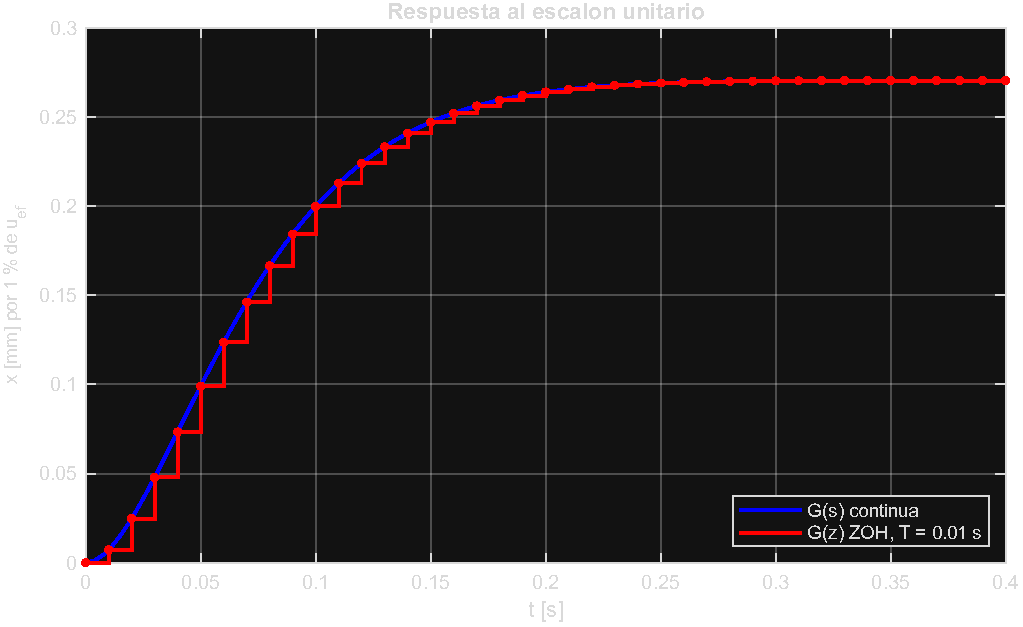
\includegraphics[width=0.75\textwidth]{escalon_continuo_discreto.pdf}
  \caption{Respuesta al escalón unitario de $G(s)$ y de $G(z)$ con ZOH. Las
           muestras de $G(z)$ caen exactamente sobre la curva continua.}
\end{figure}

\begin{figure}[H]
  \centering
  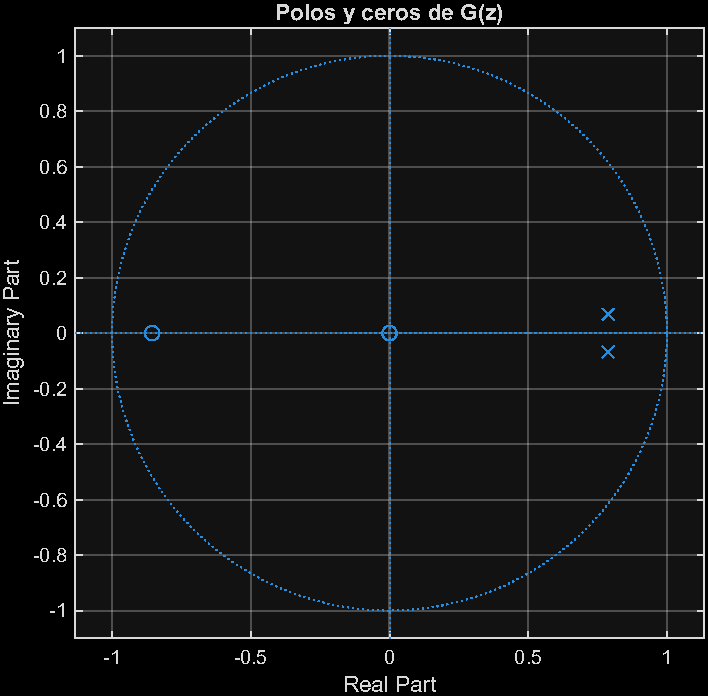
\includegraphics[width=0.5\textwidth]{polos_ceros_z.pdf}
  \caption{Polos y cero de $G(z)$ en el plano $z$.}
\end{figure}

%--------------------------------------------------------------------------
\section{Ecuación en diferencias de la planta}

De \eqref{eq:Gz}, $X(z)\,(1 - 1.576343z^{-1} + 0.625815z^{-2}) =
U_{ef}(z)\,(0.007209z^{-1} + 0.006166z^{-2})$. Antitransformando:
\begin{equation}
  \boxed{x(k) = 1.576343\,x(k-1) - 0.625815\,x(k-2)
               + 0.007209\,u_{ef}(k-1) + 0.006166\,u_{ef}(k-2)}
\end{equation}
Esta ecuación está implementada en el firmware del ESP32 como modelo de la
planta (\texttt{plant\_model\_step}) y su salida se envía en la telemetría
junto a la posición medida, para validar el modelo en tiempo real.

%==========================================================================
\section{Especificaciones del lazo cerrado}

Ambos controladores deben seguir un escalón con $e_{ss}=0$. Para compararlos
en igualdad de condiciones se usa el mismo polinomio deseado:
\begin{align}
  \zeta_d &= \zetad \quad\text{(sin sobrepico)}, &
  t_{s,d} &= \tsd~\text{s}, &
  \omega_{n,d} &= \frac{4}{\zeta_d\,t_{s,d}} = \frac{4}{(1)(\tsd)} = \wnd~\text{rad/s}
\end{align}
Como la planta es de segundo orden y el PID agrega un polo en el origen, el
lazo cerrado es de tercer orden. El tercer polo se ubica en
\begin{equation}
  p_3 = 5\,\zeta_d\,\omega_{n,d} = \pthree~\text{rad/s}.
\end{equation}
En la práctica 3 se usó $p_3 = 10\zeta\omega_n$; aquí eso da
$p_3 T = 1.33$, y al discretizar con Euler el lazo pierde la forma continua
(sobrepico de $28.6\,\%$ en la simulación lineal). Con $5\zeta\omega_n$,
$p_3 T = 0.67$ y la respuesta discreta conserva la continua con la mitad de
ganancia, lo que además reduce el efecto del ruido de cuantización del encoder.

El tiempo de muestreo se mantiene en $T = 0.01$~s: con el lazo cerrado
$t_{s,d}/T = 30$, más fino que el rango $t_s/20$--$t_s/10$, lo que es
conservador.

%==========================================================================
\section{Controlador PID continuo--discreto}

\subsection{Diseño continuo por asignación de polos}
Con $C(s) = \dfrac{K_d s^2 + K_p s + K_i}{s}$ y
$G(s) = \dfrac{b_0}{s^2 + a_1 s + a_0}$ ($b_0=168.4$, $a_1=46.87$, $a_0=622.9$),
la ecuación característica $1 + C(s)G(s) = 0$ es
\begin{equation}
  s^3 + (a_1 + b_0 K_d)\,s^2 + (a_0 + b_0 K_p)\,s + b_0 K_i = 0 .
\end{equation}
El polinomio deseado es
\begin{align}
  P_d(s) &= \bigl(s^2 + 2\zeta_d\omega_{n,d}\,s + \omega_{n,d}^2\bigr)(s + p_3)
  = (s^2 + 26.6667\,s + 177.7778)(s + \pthree) \nonumber\\
  &= s^3 + \PdsA\,s^2 + \PdsB\,s + \PdsC
\end{align}
Igualando coeficientes:
\begin{align}
  K_d &= \frac{\PdsA - 46.87}{168.4} = \Kd\\
  K_p &= \frac{\PdsB - 622.9}{168.4} = \Kp\\
  K_i &= \frac{\PdsC}{168.4} = \Ki
\end{align}

\subsection{Discretización por Euler hacia atrás}
Con $s = \dfrac{1 - z^{-1}}{T}$:
\begin{equation}
  C(z) = \frac{\dfrac{K_d}{T}(1-z^{-1})^2 + K_p(1-z^{-1}) + K_i T}{1 - z^{-1}}
       = \frac{q_0 + q_1 z^{-1} + q_2 z^{-2}}{1 - z^{-1}}
\end{equation}
\begin{align}
  q_0 &= \frac{K_d}{T} + K_p + K_i T = \KdT + \Kp + \KiT = \qcdA\\
  q_1 &= -\frac{2K_d}{T} - K_p = -2(\KdT) - \Kp = \qcdB\\
  q_2 &= \frac{K_d}{T} = \qcdC
\end{align}
\begin{equation}
  \boxed{u(k) = u(k-1) + \qcdA\,e(k) \qcdB\,e(k-1) + \qcdC\,e(k-2)}
\end{equation}
La suma $q_0+q_1+q_2 = K_i T = \KiT$ es la ganancia integral por muestra; el
polo en $z=1$ garantiza $e_{ss}=0$ ante escalón.

%==========================================================================
\section{Controlador discreto--discreto}

\subsection{Estructura}
Sobre la planta discreta
$G(z) = \dfrac{b_1 z^{-1} + b_2 z^{-2}}{1 + a_1 z^{-1} + a_2 z^{-2}}$ se usa
\begin{equation}
  C(z) = \frac{q_0 + q_1 z^{-1} + q_2 z^{-2}}{(1 - z^{-1})(1 + s_0 z^{-1})},
\end{equation}
con integrador ($z=1$) para $e_{ss}=0$. Hay cuatro incógnitas
($q_0,q_1,q_2,s_0$) y la ecuación característica
\begin{equation}
  A(z)\,(1 - z^{-1})(1 + s_0 z^{-1}) + B(z)\,Q(z) = P_d(z)
  \label{eq:diofantica}
\end{equation}
es de cuarto orden en $z^{-1}$.

\subsection{Polinomio deseado en $z$}
El par dominante se mapea con $z = e^{sT}$:
\begin{align}
  P_1 &= -2\,e^{-\zeta_d\omega_{n,d}T}\cos\!\bigl(\omega_{n,d}T\sqrt{1-\zeta_d^2}\bigr)
       = -2(\ezwT)(1) = \PzA\\
  P_2 &= e^{-2\zeta_d\omega_{n,d}T} = \PzB
\end{align}
y los dos polos restantes en $\alpha = e^{-p_3 T} = e^{-0.6667} = \alfa$
(el mismo tercer polo del diseño continuo):
\begin{align}
  P_d(z) &= (1 \PzA\,z^{-1} + \PzB\,z^{-2})(1 - \alfa\,z^{-1})^2 \nonumber\\
         &= 1 \dA\,z^{-1} + \dB\,z^{-2} \dC\,z^{-3} + \dD\,z^{-4}
\end{align}

\subsection{Igualación de coeficientes}
Primero
$A(z)(1-z^{-1}) = (1 - 1.576343z^{-1} + 0.625815z^{-2})(1 - z^{-1})
= 1 \ADA\,z^{-1} + \ADB\,z^{-2} \ADC\,z^{-3}$.
Multiplicando por $(1+s_0z^{-1})$, sumando $B(z)Q(z)$ e igualando con
$P_d(z)$ potencia por potencia:
\begin{align}
  z^{-1}:&\quad \ADA + s_0 + b_1 q_0 = \dA\\
  z^{-2}:&\quad \ADB \ADA\,s_0 + b_2 q_0 + b_1 q_1 = \dB\\
  z^{-3}:&\quad \ADC + \ADB\,s_0 + b_2 q_1 + b_1 q_2 = \dC\\
  z^{-4}:&\quad \ADC\,s_0 + b_2 q_2 = \dD
\end{align}
con $b_1 = 0.007209$ y $b_2 = 0.006166$. En forma matricial
\begin{equation}
\begin{bmatrix}
 0.007209 & 0 & 0 & 1\\
 0.006166 & 0.007209 & 0 & \ADA\\
 0 & 0.006166 & 0.007209 & \ADB\\
 0 & 0 & 0.006166 & \ADC
\end{bmatrix}
\begin{bmatrix} q_0\\ q_1\\ q_2\\ s_0 \end{bmatrix}
=
\begin{bmatrix} \dA - (\ADA)\\ \dB - \ADB\\ \dC - (\ADC)\\ \dD \end{bmatrix}
\end{equation}
y resolviendo:
\begin{equation}
  q_0 = \qddA,\qquad q_1 = \qddB,\qquad q_2 = \qddC,\qquad s_0 = \sdd
\end{equation}

\subsection{Ecuación en diferencias}
Como $(1 - z^{-1})(1 + s_0z^{-1}) = 1 + (s_0 - 1)z^{-1} - s_0 z^{-2}$:
\begin{equation}
  \boxed{u(k) = \oneMinusSdd\,u(k-1) \sdd\,u(k-2) + \qddA\,e(k) \qddB\,e(k-1) + \qddC\,e(k-2)}
\end{equation}

%==========================================================================
\section{Simulación en Simulink}

El modelo \texttt{simulacion/lab5\_control.slx} (figura~\ref{fig:sl}) tiene
tres lazos con la misma referencia ($+5$~mm en $t=0.1$~s y $-5$~mm en
$t=1.6$~s):
\begin{itemize}
  \item \textbf{PID continuo}: el diseño ideal, sin saturación (referencia).
  \item \textbf{Continuo--discreto} y \textbf{discreto--discreto}: la ecuación
        en diferencias con retardos unitarios $z^{-1}$, muestreo de $r$ y $y$
        con ZOH ($T=0.01$~s), saturación del actuador
        ($\Umin \le u_{ef} \le \Umax~\%$, lo que queda del PWM después de la
        zona muerta) y un cuantizador de $0.0671$~mm que representa el encoder.
  \item El ISE se obtiene integrando $e^2$.
\end{itemize}
Los retardos de $u$ guardan el valor sin saturar: el controlador es lineal y
solo se satura su salida. Con el valor saturado en la memoria, el término
$q_1 e(k-1)$ del PID con derivativo provoca una subida inversa de $-1.1$~mm
después de cada escalón.

\begin{figure}[H]
  \centering
  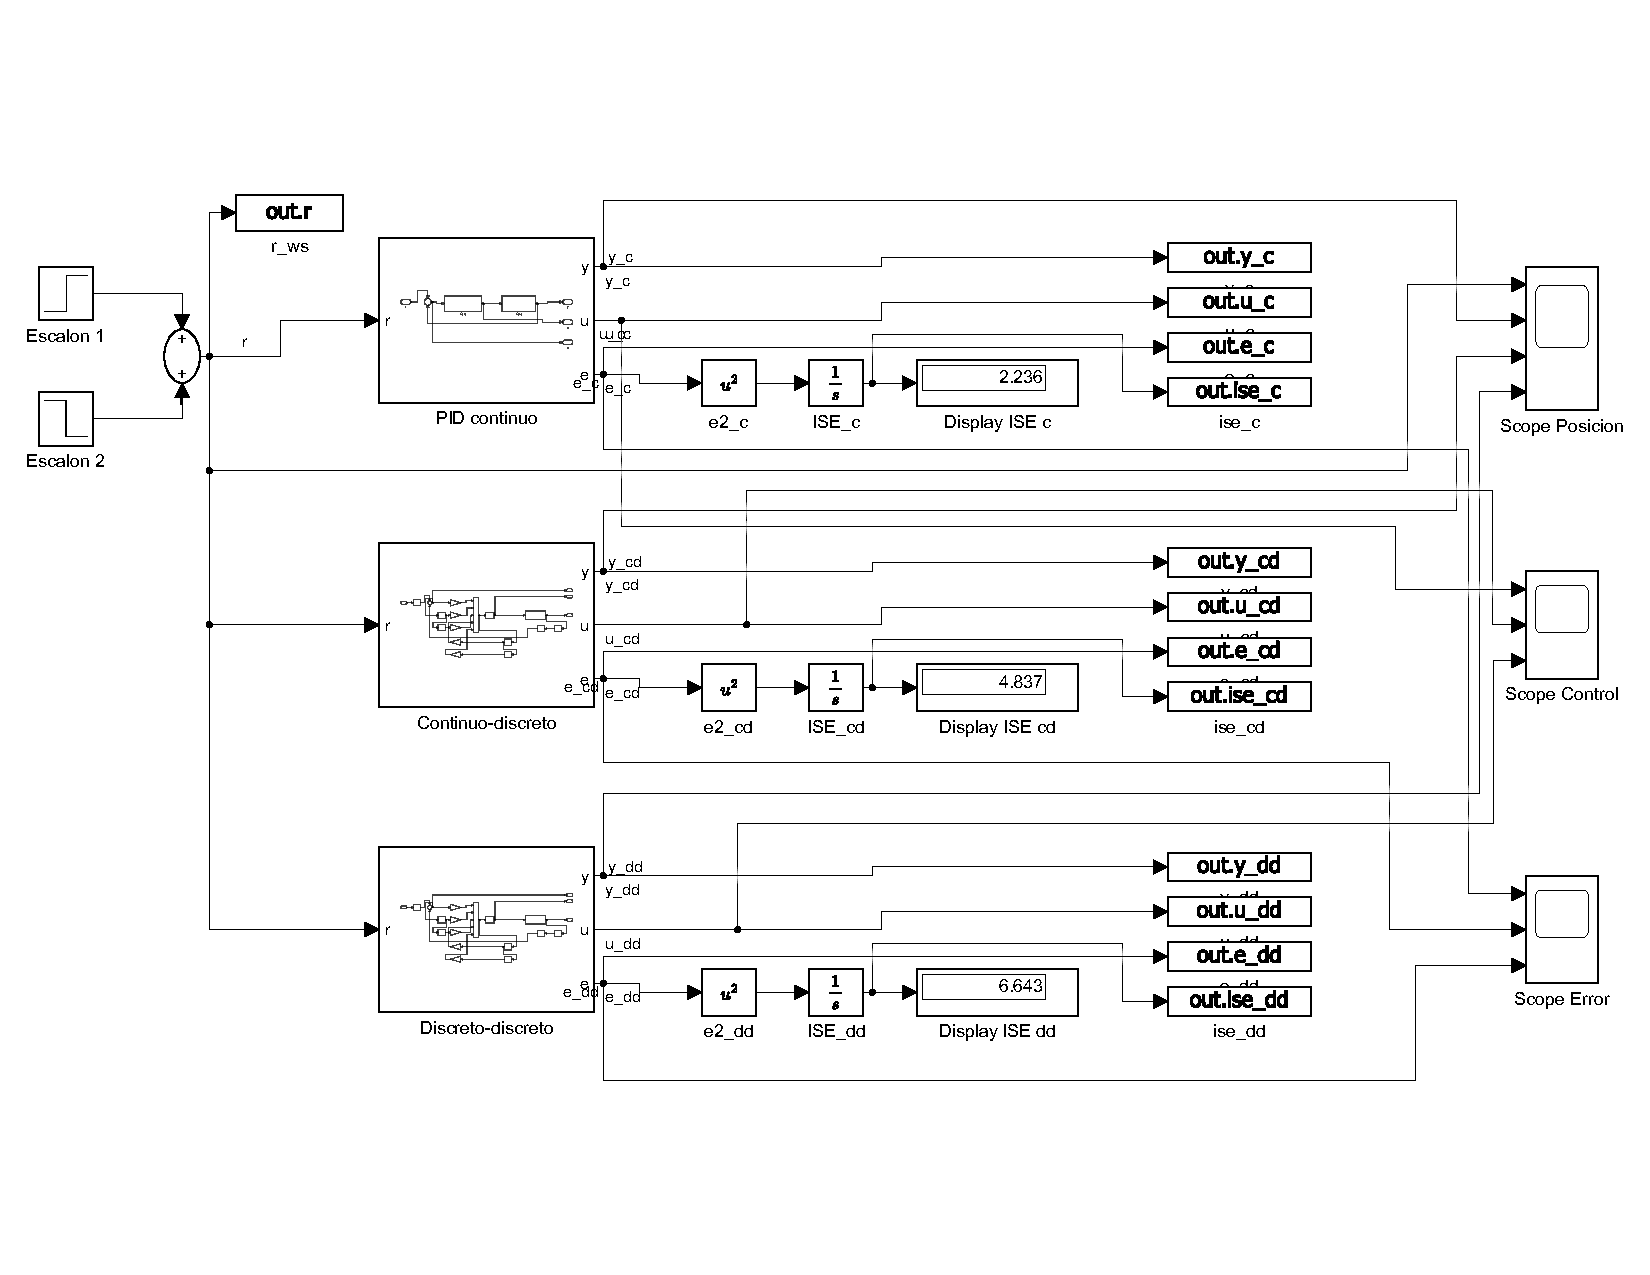
\includegraphics[width=\textwidth]{simulink_modelo.pdf}
  \caption{Modelo de Simulink.}
  \label{fig:sl}
\end{figure}
\begin{figure}[H]
  \centering
  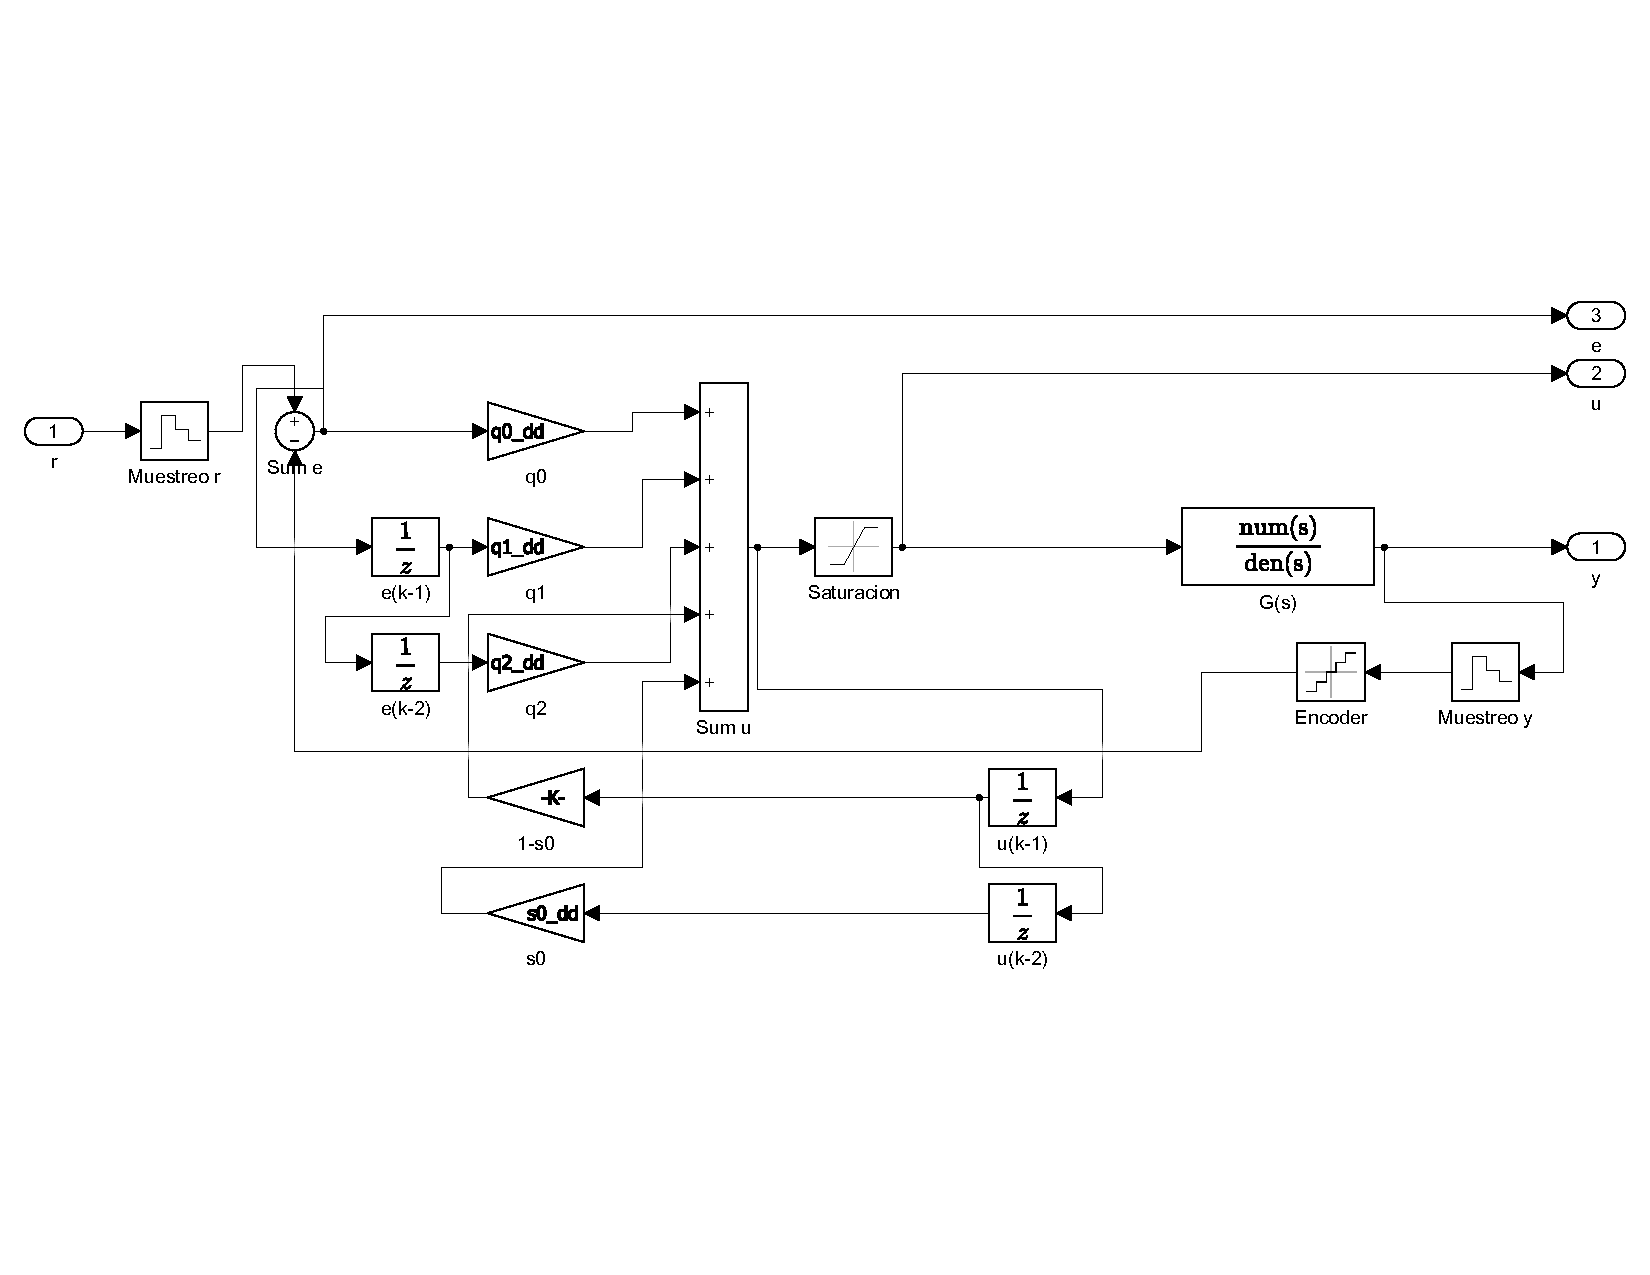
\includegraphics[width=\textwidth]{simulink_lazo_discreto.pdf}
  \caption{Lazo discreto: ecuación en diferencias, saturación, planta y encoder.}
\end{figure}

\begin{table}[H]
\centering
\begin{tabular}{lcccccc}
\toprule
 & \multicolumn{3}{c}{Escalón $0 \to +5$ mm} & \multicolumn{3}{c}{Escalón $+5 \to -5$ mm}\\
\cmidrule(lr){2-4}\cmidrule(lr){5-7}
Controlador & $t_s$ [s] & $M_p$ [\%] & ISE & $t_s$ [s] & $M_p$ [\%] & ISE\\
\midrule
PID continuo (ideal)  & \maAts & \maAmp & \maAise & \maBts & \maBmp & \maBise\\
Continuo--discreto    & \mbAts & \mbAmp & \mbAise & \mbBts & \mbBmp & \mbBise\\
Discreto--discreto    & \mcAts & \mcAmp & \mcAise & \mcBts & \mcBmp & \mcBise\\
\bottomrule
\end{tabular}
\caption{Resultados de simulación (ISE en mm$^2\cdot$s). En todos los casos
$e_{ss} \approx 0$.}
\end{table}

\begin{figure}[H]
  \centering
  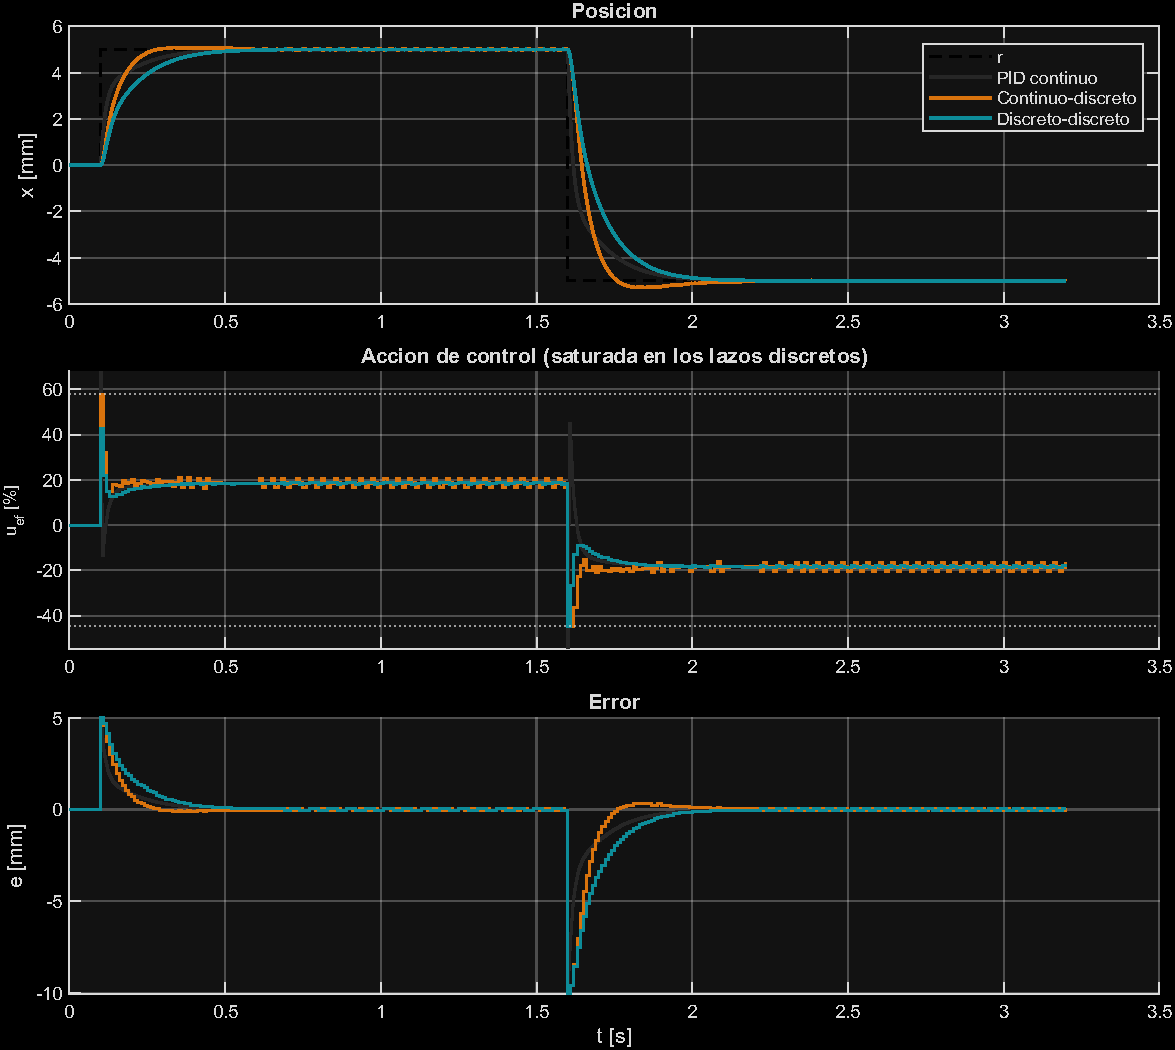
\includegraphics[width=0.95\textwidth]{sim_respuestas.pdf}
  \caption{Posición, acción de control y error simulados.}
\end{figure}
\begin{figure}[H]
  \centering
  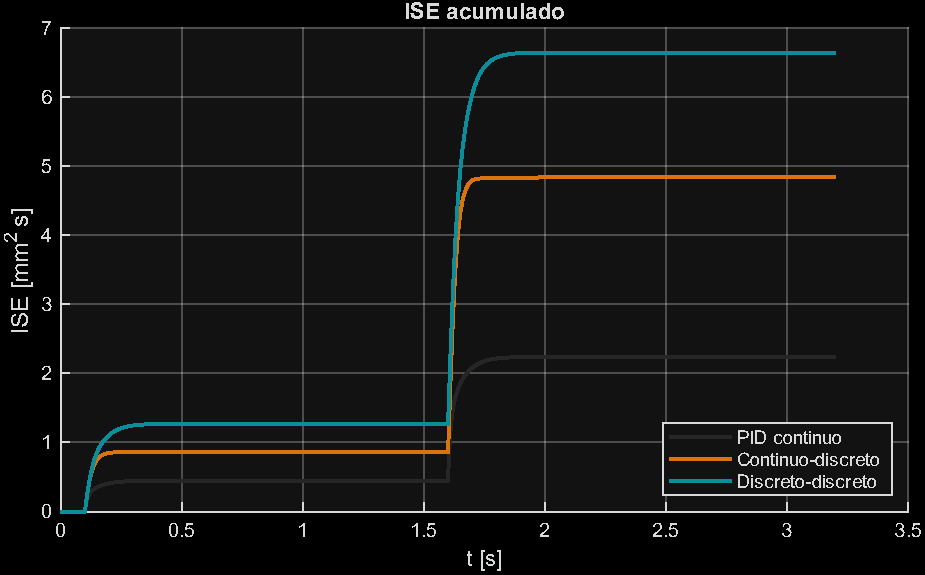
\includegraphics[width=0.7\textwidth]{sim_ise.pdf}
  \caption{ISE acumulado.}
\end{figure}

El PID continuo ideal es el más rápido porque no tiene límite en la acción de
control (llega a $\pm1357~\%$ por el derivativo). Con saturación, el
continuo--discreto responde más rápido y con menor ISE, a cambio de un
sobrepico pequeño ($<3~\%$) y de saturar el actuador al inicio de cada
escalón ($q_0 = \qcdA$ multiplica directamente el escalón de error). El
discreto--discreto tiene ganancias unas cuatro veces menores ($q_0 = \qddA$),
casi no satura, no tiene sobrepico y sus polos de lazo cerrado son
exactamente los deseados, pero es más lento y acumula más ISE.

%==========================================================================
\section{Implementación en el ESP32}

Cada $T = 10$~ms el firmware lee el encoder, calcula $e(k) = r(k) - y(k)$,
evalúa la ecuación en diferencias del controlador activo, satura $u_{ef}$ y
suma la zona muerta del lado correspondiente antes de aplicar el PWM al
L298N:
\begin{lstlisting}[language=C]
static float ctrl_step(ctrl_state_t *st, const ctrl_coef_t *c, float e)
{
    float u = (1.0f - c->s0) * st->u1 + c->s0 * st->u2
            + c->q0 * e + c->q1 * st->e1 + c->q2 * st->e2;
    u = clampf(u, -U_MEM_LIMIT, U_MEM_LIMIT);
    st->e2 = st->e1;  st->e1 = e;
    st->u2 = st->u1;  st->u1 = u;
    return clampf(u, U_EF_MIN, U_EF_MAX);   // u_ef saturado
}
\end{lstlisting}
La interfaz web (\texttt{app/}) se comunica por USB serial: grafica $r$, $y$,
$e$ y $u$ en tiempo real, cambia la referencia, calcula el ISE en una ventana
deslizante, ejecuta pruebas de escalón automáticas para comparar los dos
controladores y guarda los datos con el tiempo de muestreo en CSV.

\begin{figure}[H]
  \centering
  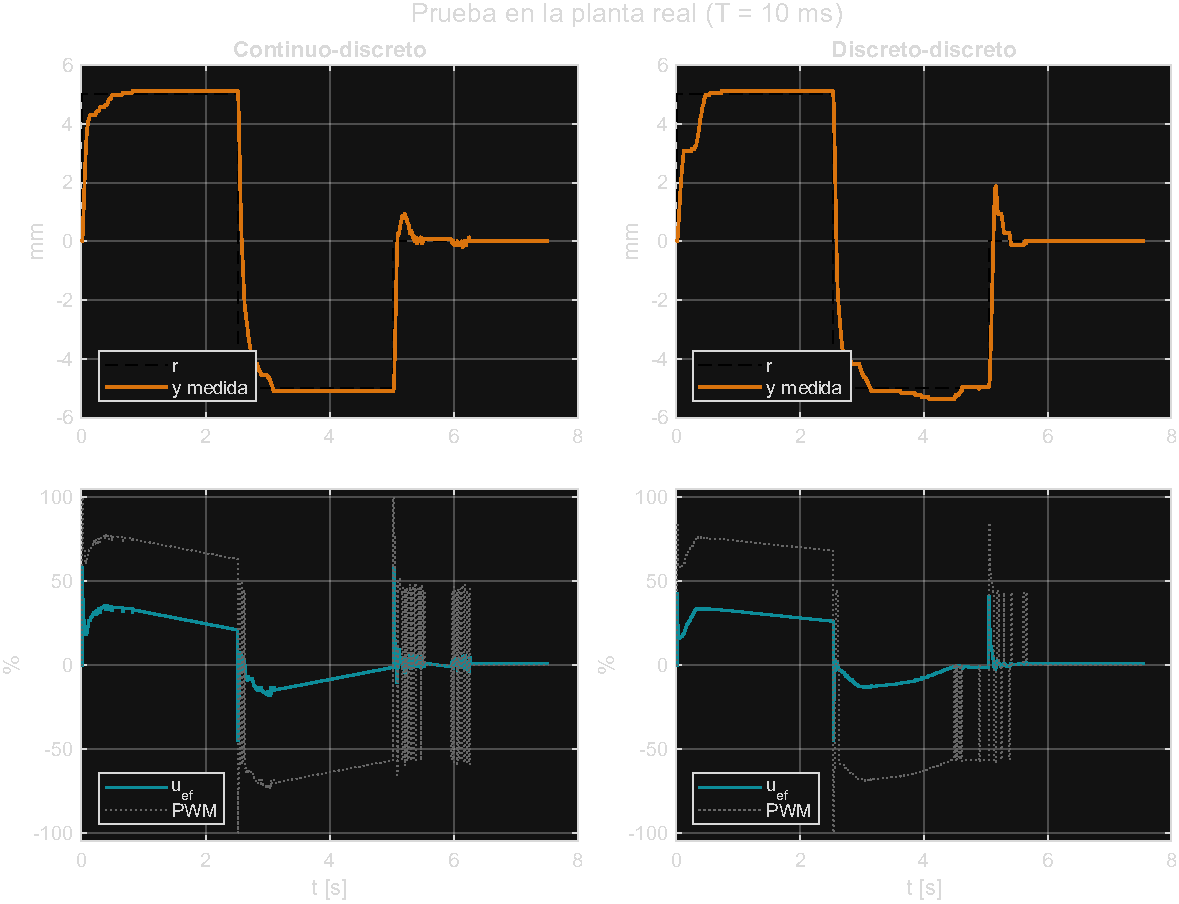
\includegraphics[width=0.95\textwidth]{real_lazo.pdf}
  \caption{Prueba preliminar sobre la planta real: escalones $0\to5\to-5\to0$~mm.}
\end{figure}

En la prueba preliminar ambos controladores llevan la masa a la referencia y
el error final queda en $\pm0.10$~mm (1.5 cuentas del encoder): la fricción
estática retiene la masa dentro de esa banda mientras la acción integral
crece lentamente.

\end{document}
